\documentclass[12pt,a4paper,oneside]{report}

% -------------------------------------------------------------
% IIT Indore Report Formatting Packages (reportbtp.pdf)
% -------------------------------------------------------------
\usepackage[utf8]{inputenc}
\usepackage[left=1.25in,right=1.0in,top=1.0in,bottom=1.0in]{geometry}
\usepackage{times}              % Times New Roman typography
\usepackage{setspace}
\onehalfspacing                 % 1.5 line spacing mandated by IIT Indore
\usepackage{graphicx}
\usepackage{amsmath,amssymb}
\usepackage{booktabs}
\usepackage{array}
\usepackage{caption}
\usepackage{subcaption}
\usepackage{listings}
\usepackage{xcolor}
\usepackage{cite}
\usepackage[colorlinks=true,linkcolor=black,citecolor=blue,urlcolor=NavyBlue]{hyperref}

\definecolor{NavyBlue}{RGB}{0,32,96}

% Listings formatting for assembly and Python code
\lstset{
    frame=single,
    basicstyle=\ttfamily\footnotesize,
    keywordstyle=\color{NavyBlue}\bfseries,
    commentstyle=\color{gray}\textit,
    stringstyle=\color{purple},
    numbers=left,
    numberstyle=\tiny\color{gray},
    breaklines=true,
    showstringspaces=false,
    tabsize=4
}

\begin{document}

% -------------------------------------------------------------
% Front Matter
% -------------------------------------------------------------
% Front Matter conforming to IIT Indore BTP Guidelines (reportbtp.pdf)

% -------------------------------------------------------------
% COVER PAGE (Page 2 of reportbtp.pdf sample)
% -------------------------------------------------------------
\begin{titlepage}
\centering
\vspace*{0.5cm}
{\huge \textbf{B. TECH. PROJECT REPORT}\par}
\vspace{1.0cm}
{\Large \textit{On}\par}
\vspace{1.0cm}
{\huge \textbf{\textcolor{NavyBlue}{Emerging Fault Analysis Techniques of Lightweight Ciphers}}\par}
\vspace{2.5cm}
{\Large \textbf{BY}\par}
\vspace{0.8cm}
{\LARGE \textbf{Milkuri Raja Reddy (230001054)}\par}
\vspace{0.3cm}
{\LARGE \textbf{Dharavath Vikas (230002023)}\par}
\vfill
{\Large \textbf{DISCIPLINE OF COMPUTER SCIENCE AND ENGINEERING}\par}
\vspace{0.4cm}
{\Large \textbf{INDIAN INSTITUTE OF TECHNOLOGY INDORE}\par}
\vspace{0.4cm}
{\Large \textbf{November 2026}\par}
\vspace*{0.5cm}
\end{titlepage}

\cleardoublepage

% -------------------------------------------------------------
% TITLE PAGE (Page 3 of reportbtp.pdf sample)
% -------------------------------------------------------------
\begin{titlepage}
\centering
\vspace*{0.5cm}
{\huge \textbf{Emerging Fault Analysis Techniques of Lightweight Ciphers}\par}
\vspace{1.5cm}
{\Large \textbf{A PROJECT REPORT}\par}
\vspace{0.5cm}
{\large \textit{Submitted in partial fulfillment of the requirements for the award of the degree of}\par}
\vspace{0.3cm}
{\large \textit{of}\par}
\vspace{0.3cm}
{\Large \textbf{BACHELOR OF TECHNOLOGY}\par}
\vspace{0.3cm}
{\large \textit{in}\par}
\vspace{0.3cm}
{\Large \textbf{COMPUTER SCIENCE AND ENGINEERING}\par}
\vspace{1.5cm}
{\large \textit{Submitted by:}\par}
\vspace{0.3cm}
{\Large \textbf{Milkuri Raja Reddy (230001054)}\par}
\vspace{0.2cm}
{\Large \textbf{Dharavath Vikas (230002023)}\par}
\vspace{1.5cm}
{\large \textit{Guided by:}\par}
\vspace{0.3cm}
{\Large \textbf{Prof. Bodhisatwa Mazumdar}\par}
\vspace{0.2cm}
{\large Department of Computer Science and Engineering\par}
\vfill
{\Large \textbf{INDIAN INSTITUTE OF TECHNOLOGY INDORE}\par}
\vspace{0.3cm}
{\Large \textbf{November 2026}\par}
\vspace*{0.5cm}
\end{titlepage}

\cleardoublepage
\pagenumbering{roman}
\setcounter{page}{4}

% -------------------------------------------------------------
% CANDIDATE'S DECLARATION & CERTIFICATE (Page 4 of reportbtp.pdf)
% -------------------------------------------------------------
\chapter*{Candidate's Declaration}
\addcontentsline{toc}{chapter}{Candidate's Declaration}

We hereby declare that the project entitled \textbf{``Emerging Fault Analysis Techniques of Lightweight Ciphers''} submitted in partial fulfillment for the award of the degree of Bachelor of Technology in `\textbf{Computer Science and Engineering}' completed under the supervision of \textbf{Prof. Bodhisatwa Mazumdar}, Department of Computer Science and Engineering, IIT Indore is an authentic work carried out by us.

\noindent
Further, we declare that we have not submitted this work for the award of any other degree or diploma elsewhere.

\vspace{2.5cm}
\noindent
\begin{tabular*}{\textwidth}{@{\extracolsep{\fill}}ll}
\rule{6.5cm}{0.4pt} & \rule{6.5cm}{0.4pt} \\
\textbf{Milkuri Raja Reddy (230001054)} & \textbf{Dharavath Vikas (230002023)} \\
B.Tech. IV Year & B.Tech. IV Year \\
Department of CSE, IIT Indore & Department of CSE, IIT Indore \\
Date: November 20, 2026 & Date: November 20, 2026 \\
\end{tabular*}

\vspace{1.5cm}
\noindent
\rule{\textwidth}{1.0pt}
\vspace{0.5cm}

\section*{CERTIFICATE by BTP Guide(s)}

It is certified that the above statement made by the students \textbf{Milkuri Raja Reddy (230001054)} and \textbf{Dharavath Vikas (230002023)} is correct to the best of my knowledge and belief.

\vspace{2.5cm}
\noindent
\begin{tabular}{l}
\rule{7.0cm}{0.4pt} \\
\textbf{Prof. Bodhisatwa Mazumdar} \\
Professor, Department of Computer Science and Engineering \\
Indian Institute of Technology Indore \\
Date: November 20, 2026 \\
\end{tabular}

\cleardoublepage

% -------------------------------------------------------------
% PREFACE (Page 5 of reportbtp.pdf)
% -------------------------------------------------------------
\chapter*{Preface}
\addcontentsline{toc}{chapter}{Preface}

This report on \textbf{``Emerging Fault Analysis Techniques of Lightweight Ciphers''} is prepared under the guidance of \textbf{Prof. Bodhisatwa Mazumdar}, Department of Computer Science and Engineering, Indian Institute of Technology Indore.

Lightweight block ciphers are widely deployed in modern Cyber-Physical Systems (CPS), smart cards, and Internet-of-Things (IoT) edge microcontrollers. Due to severe constraints on silicon area and power budgets, newly proposed lightweight ciphers frequently adopt low-degree algebraic structures and simplified key schedules to minimize Threshold Implementation (TI) masking overheads. A prime example is \textbf{BAKSHEESH} (Baksi et al., 2023), introduced as an area-efficient alternative to GIFT-128. While BAKSHEESH successfully achieves a $2.43\times$ reduction in masked hardware area over GIFT-128, the designers explicitly made no claims regarding physical fault resistance.

Through this report, we evaluate the vulnerability of emerging lightweight block ciphers against \textbf{Linked Fault Analysis (LFA)} (Beigizad et al., IEEE TIFS 2024). We analyze:
\begin{enumerate}
    \item \textbf{Linked Differential Fault Analysis (LDFA)} on unprotected implementations, recovering the full 128-bit key in exactly 31 faults in Round 35.
    \item \textbf{Linked Ineffective Fault Analysis (LIFA)} on hardened implementations, proving that duplicate-and-compare redundancy countermeasures are fundamentally bypassed with an average of only 508.9 queries.
    \item \textbf{Physical Realism Enhancements}: Demonstrating blind identification across all $\binom{32}{2} = 496$ candidate pairs with $100\%$ accuracy for $N \ge 5$, and proving key recovery resilience against glitch miss noise up to $p_{\text{miss}} = 30\%$.
    \item \textbf{Cycle-Accurate RISC-V Hardware Modeling}: Validating instruction-skip fault injection in bare-metal RV32I assembly on the RARS simulator.
    \item \textbf{Unified Lightweight Countermeasures}: Proposing, implementing, and empirically validating a combined SCA (3-share TI) and LFA-resistant architecture that completely neutralizes both LDFA and LIFA attacks.
\end{enumerate}

\vspace{1.5cm}
\noindent
\textbf{Milkuri Raja Reddy (230001054)} \\
\textbf{Dharavath Vikas (230002023)} \\
B.Tech. IV Year, Discipline of Computer Science and Engineering \\
Indian Institute of Technology Indore

\cleardoublepage

% -------------------------------------------------------------
% ACKNOWLEDGEMENTS (Page 6 of reportbtp.pdf)
% -------------------------------------------------------------
\chapter*{Acknowledgements}
\addcontentsline{toc}{chapter}{Acknowledgements}

We wish to express our profound gratitude and respect to our project supervisor, \textbf{Prof. Bodhisatwa Mazumdar}, Department of Computer Science and Engineering, Indian Institute of Technology Indore, for his kind support, valuable guidance, and inspiring mentorship throughout this B.Tech. Project. It is his deep domain expertise in hardware security, side-channel analysis, cryptographic implementations, and physical fault injection, due to which we became able to complete the theoretical foundations, microarchitectural assembly simulations, empirical attack pipelines, and this comprehensive technical report. Without his continuous support and encouragement, this work would not have been possible.

We would also like to thank the Head of the Department and all faculty members of the Department of Computer Science and Engineering at IIT Indore for providing computational facilities, access to academic resources, and an enriching research environment.

We express our gratitude to our peers and lab colleagues in the Hardware Security and Cryptography group for their engaging discussions and constructive critiques during our experimental evaluations.

Lastly, we express our heartfelt appreciation to our parents, family members, and friends for their continuous patience, motivation, and moral support throughout our undergraduate journey.

\vspace{1.5cm}
\noindent
\textbf{Milkuri Raja Reddy (230001054)} \\
\textbf{Dharavath Vikas (230002023)} \\
Department of Computer Science and Engineering \\
Indian Institute of Technology Indore

\cleardoublepage

% -------------------------------------------------------------
% ABSTRACT (Page 7 of reportbtp.pdf)
% -------------------------------------------------------------
\chapter*{Abstract}
\addcontentsline{toc}{chapter}{Abstract}

Lightweight block ciphers form the foundational cryptographic backbone of resource-constrained embedded systems, smart sensing dust, and autonomous Internet-of-Things (IoT) edge appliances. The lightweight block cipher \textbf{BAKSHEESH} was recently introduced as an area-efficient alternative to GIFT-128, utilizing an involution-based 4-bit S-Box with a non-trivial linear structure and a full 128-bit round key injection driven by a single 1-bit rotational key schedule. Although this design achieves a $2.43\times$ hardware area reduction under Threshold Implementation (TI) Boolean masking, the cipher does not incorporate inherent protection against physical fault injection.

In this B.Tech. Project Report, we present a comprehensive mathematical, empirical, and microarchitectural evaluation of emerging lightweight block ciphers under \textbf{Linked Fault Analysis (LFA)}:
\begin{enumerate}
    \item \textbf{Linked Differential Fault Analysis (LDFA)}: In unprotected implementations, we demonstrate that injecting linked equality faults ($u' = v$) across adjacent nibbles in the final SubCells layer (Round 35) directly leaks equivalent subkey (ESK) differences. Across 31 adjacent nibble pairs, LDFA collapses the $2^{128}$ key search space down to only 16 candidate keys ($2^4$), uniquely resolved using a single known plaintext-ciphertext pair.
    \item \textbf{Linked Ineffective Fault Analysis (LIFA)}: In hardened implementations fortified with spatial redundancy countermeasures (duplicate-and-compare), effective faults are caught and suppressed. However, when the two linked nibbles are naturally identical ($x[i] == x[j]$), the fault induces zero functional modification ($y[i] == y[j]$). This \textbf{ineffective fault completely bypasses the redundancy check}, emitting a valid ciphertext that directly leaks the subkey difference $\Delta esk[i, j]$. We prove that an empirical average of \textbf{508.9 queries} (theoretical expectation: 496.0 queries) achieves full 128-bit key recovery with a 100\% success rate.
    \item \textbf{Architectural Comparison with GIFT-128}: We establish that while BAKSHEESH is fully broken in 1 round (31 faults / 508.9 queries), GIFT-128 requires attacking two consecutive rounds (Rounds 39 and 40) due to its 64-bit narrow key injection. Consequently, GIFT-128 requires 62 faults (LDFA) or $\approx 1000$ queries (LIFA) and leaves a 256-candidate space ($2^8$), demonstrating an inherent architectural resilience trade-off.
    \item \textbf{Robustness to Practical Noise \& Unknown Fault Locations}: In realistic physical attack scenarios where the targeted pair is unknown, we design an automated locator that identifies the faulted nibble pair $(i, j)$ with \textbf{100.0\% accuracy for $N \ge 5$ blind ciphertexts} via majority voting over all $\binom{32}{2} = 496$ candidate pairs. Furthermore, we demonstrate that majority voting tolerates glitch miss noise up to $p_{\text{miss}} = 30\%$ with $100\%$ key recovery success across $N \le 30$ attempts per relation.
    \item \textbf{Cycle-Accurate RISC-V Hardware Validation}: We implement Round 1 of BAKSHEESH in bare-metal RV32I assembly (\texttt{baksheesh\_round1.s}) and validate inside the RARS simulator that single instruction skips during the S-box substitution loop physically produce the exact linked equality relation.
    \item \textbf{Proposed Unified Countermeasures}: To mitigate LFA, we propose, implement, and benchmark a unified countermeasure suite combining explicit register zeroing (\texttt{li x31, 0}), S-box loop shuffling, and asymmetric infective dummy state diffusion. We prove that this unified architecture drops adversary attack success from 100\% to 0\% while preserving BAKSHEESH's $2.43\times$ masking advantage.
\end{enumerate}

\noindent
\textbf{Keywords}: Lightweight Cryptography, BAKSHEESH, GIFT-128, Linked Fault Analysis, Linked Ineffective Fault Analysis, Redundancy Countermeasures, Unknown Fault Location, Noise Tolerance, RISC-V RV32I, RARS, Unified Countermeasures.

\cleardoublepage


% -------------------------------------------------------------
% Table of Contents, List of Figures, List of Tables
% -------------------------------------------------------------
\tableofcontents
\cleardoublepage

\listoffigures
\addcontentsline{toc}{chapter}{List of Figures}
\cleardoublepage

\listoftables
\addcontentsline{toc}{chapter}{List of Tables}
\cleardoublepage

\pagenumbering{arabic}
\setcounter{page}{1}

% -------------------------------------------------------------
% Main Technical Chapters
% -------------------------------------------------------------
\chapter{Introduction}
\label{ch:intro}

\section{Background and Motivation}
\label{sec:background}
The rapid proliferation of Cyber-Physical Systems (CPS), smart microgrids, automotive electronic control units (ECUs), implantable biomedical electronics, and edge Internet-of-Things (IoT) sensor nodes has revolutionized modern digital infrastructure. These embedded devices process sensitive financial, personal, and operational telemetry in real time. However, unlike traditional enterprise servers and desktop workstations that operate within secure server rooms with plentiful power, edge devices operate under stringent computational, thermal, and electrical constraints. Modern edge microcontrollers frequently feature fewer than 2,000 to 5,000 logic gate equivalents (GE) dedicated to security primitives, minimal volatile SRAM, and micro-watt energy envelopes.

To satisfy these uncompromising requirements, the cryptographic research community has standardized dedicated \textbf{Lightweight Block Ciphers}. Rather than deploying heavyweight standards such as the Advanced Encryption Standard (AES)~\cite{biham1997differential}, embedded designers employ lightweight primitives like PRESENT, SIMON, SPECK, and GIFT-128~\cite{banik2017gift}. In 2023, Baksi et al.~\cite{baksi2023baksheesh} introduced \textbf{BAKSHEESH}, positioning it as ``similar yet different from GIFT-128''. BAKSHEESH adopts the general substitution-permutation network (SPN) topology of GIFT-128 but incorporates two major modifications:
\begin{enumerate}
    \item It replaces GIFT-128's degree-3 S-box with an involution-based 4-bit S-box possessing a non-trivial linear structure ($8 \to F$).
    \item It replaces GIFT-128's split LFSR-driven key schedule with a full 128-bit key injection driven by a trivial 1-bit cyclic rotation schedule.
\end{enumerate}
These architectural optimizations achieve an impressive $2.43\times$ hardware area reduction when protected against Side-Channel Analysis (SCA) using 3-share Threshold Implementation (TI) Boolean masking. However, the designers of BAKSHEESH explicitly stated in their specification that they made no claims regarding physical fault resistance.

\section{Physical Fault Attacks vs. Speculative Execution Attacks}
\label{sec:faults_vs_speculation}
In contemporary microarchitectural security, it is vital to draw a strict boundary between active physical fault injection attacks and passive transient execution side channels:
\begin{itemize}
    \item \textbf{Transient / Speculative Execution Attacks}: Microarchitectural vulnerabilities like Spectre and Meltdown~\cite{canella2020systematic} exploit speculative execution windows, out-of-order instruction scheduling, and branch prediction buffers without altering physical architectural register states. These attacks leak confidential information via timing side channels in hardware caches. Consequently, software serialization barriers and pipeline fences (such as \texttt{fence.i} in RISC-V or \texttt{lfence} in x86) are capable of suppressing transient speculation leakage.
    \item \textbf{Active Physical Fault Injection Attacks (FIA)}: Physical fault injection actively perturbs the hardware environment using clock glitches, voltage starvation, electromagnetic pulses (EMP), or focused infrared/optical laser beams. Physical fault attacks directly flip bits in silicon flip-flops, corrupt data buses, or force the processor program counter to skip instructions. \textbf{Software speculation barriers cannot prevent physical hardware bit-flips or instruction skips}, necessitating algorithmic fault-tolerant designs or hardware-level redundancy countermeasures.
\end{itemize}

\section{State-of-the-Art Fault Countermeasures}
\label{sec:countermeasures_state_of_art}
To protect cryptographic devices against classical Differential Fault Analysis (DFA)~\cite{biham1997differential}---where an adversary compares a correct ciphertext $C$ against a corrupted ciphertext $C'$ to reconstruct subkey nibbles---engineers deploy redundancy-based countermeasures:
\begin{enumerate}
    \item \textbf{Spatial Redundancy (Duplicate-and-Compare)}: The cipher is instantiated across two identical hardware cryptographic engines operating in parallel (or executed twice sequentially in software). A hardware comparator unit evaluates $C_1 \stackrel{?}{=} C_2$. If an error difference is detected, the device suppresses the ciphertext and emits a fault exception or zeroized vector.
    \item \textbf{Infective Computation}: Instead of using conditional branching (which is susceptible to branch-skipping attacks), the internal difference between redundant paths is algebraically multiplied with an error diffusion matrix to randomize or ``infect'' the ciphertext before output emission.
\end{enumerate}
Under both defensive models, classical DFA is completely thwarted because the adversary is denied access to faulty ciphertexts.

\section{Research Objectives and Core Contributions}
\label{sec:contributions}
This B.Tech. Project investigates the vulnerability of emerging lightweight block ciphers under the newly proposed \textbf{Linked Fault Analysis (LFA)} paradigm~\cite{beigizad2024linked}. LFA exploits structural dependencies where an injected fault forces an intermediate state variable $u'$ to link to another intermediate variable $v$ ($u' = l(v)$).

The major contributions of this report are organized as follows:
\begin{enumerate}
    \item \textbf{Full Mathematical Formulation of LDFA}: We establish that 31 adjacent-pair linked faults in Round 35 of BAKSHEESH directly yield equivalent subkey differences $\Delta esk[i, i+1]$, collapsing the master key space from $2^{128}$ down to 16 candidates ($2^4$), resolved with 1 verification pair.
    \item \textbf{Defeating Redundancy Countermeasures via LIFA}: We prove that when $x[i] == x[j]$, the linked fault induces zero state change ($y[i] == y[j]$). This ineffective fault passes through duplicate-and-compare circuits undetected, emitting a valid ciphertext that leaks $\Delta esk[i, j]$ with an empirical mean of 508.9 queries.
    \item \textbf{Comparative Security Analysis with GIFT-128}: We demonstrate that GIFT-128 requires attacking two consecutive rounds (Rounds 39 and 40) due to its 64-bit key injection, requiring 62 faults (LDFA) or $\approx 1000$ queries (LIFA) and leaving 256 candidates, proving an architectural trade-off between key schedule width and fault resilience.
    \item \textbf{Physical Realism: Blind Fault Localization \& Noise Tolerance}: We design and validate an automated locator that identifies the unknown faulted pair $(i, j)$ with 100\% accuracy for $N \ge 5$ blind ciphertexts across all 496 candidates, and prove that majority voting tolerates glitch miss noise up to $p_{\text{miss}} = 30\%$.
    \item \textbf{Cycle-Accurate RISC-V Hardware Modeling}: We design a bare-metal RV32I assembly model (\texttt{baksheesh\_round1.s}) in RARS, demonstrating that physical instruction skips in the S-box substitution loop physically execute the linked equality condition.
    \item \textbf{Unified Lightweight Countermeasures}: We propose, implement, and benchmark a complete defensive architecture (register zeroing, loop shuffling, and infective diffusion) that drops adversary success from 100\% to 0\%.
\end{enumerate}

\section{Organization of the Report}
\label{sec:organization}
The remainder of this report is organized as follows: Chapter~\ref{ch:ciphers} specifies the architectural details of BAKSHEESH and GIFT-128. Chapter~\ref{ch:lfa} establishes the mathematical framework of Linked Fault Analysis (LDFA and LIFA). Chapter~\ref{ch:riscv} details the cycle-accurate RISC-V assembly simulation. Chapter~\ref{ch:results} provides the empirical experimental results, blind fault identification scaling, noise tolerance, and comparative evaluations. Chapter~\ref{ch:countermeasures} details the proposed unified countermeasures and future work, followed by References and Appendices.

\chapter{Target Cipher Specifications \& Architectures}
\label{ch:ciphers}

\section{The BAKSHEESH Block Cipher}
\label{sec:baksheesh_spec}
BAKSHEESH~\cite{baksi2023baksheesh} is an iterative lightweight Substitution-Permutation Network (SPN) operating on a 128-bit block with a 128-bit master key. It executes \textbf{35 identical rounds}, followed by a post-whitening key addition. The 128-bit state $X$ is partitioned into 32 four-bit nibbles:
\begin{equation}
    X = (w_{31} \parallel w_{30} \parallel \dots \parallel w_1 \parallel w_0), \quad w_i \in \mathbb{F}_2^4
\end{equation}

\subsection{Round Function Pipeline}
Each round $r \in \{1, 2, \dots, 35\}$ applies four consecutive transformations:
\begin{enumerate}
    \item \textbf{SubCells}: Applies the identical 4-bit S-Box $S$ independently to all 32 nibbles:
    \begin{equation}
        w_i \leftarrow S[w_i], \quad 0 \le i \le 31
    \end{equation}
    \item \textbf{PermBits}: Applies the GIFT-128 bit permutation $P_{128}$ to the 128 bits of the state:
    \begin{equation}
        b_{P_{128}(k)} \leftarrow b_k, \quad 0 \le k \le 127
    \end{equation}
    where $P_{128}(k) = 4 \lfloor k / 16 \rfloor + 32 ((k \pmod{16}) \pmod 4) + \lfloor (k \pmod{16}) / 4 \rfloor$.
    \item \textbf{AddConstants}: A 6-bit round constant generated by an affine LFSR is XORed into specified state tap positions $\{8, 13, 19, 35, 67, 106\}$.
    \item \textbf{AddRoundKey}: The full 128-bit round subkey $K_r$ is XORed across the entire state:
    \begin{equation}
        X \leftarrow X \oplus K_r
    \end{equation}
\end{enumerate}

\begin{figure}[!htbp]
\centering
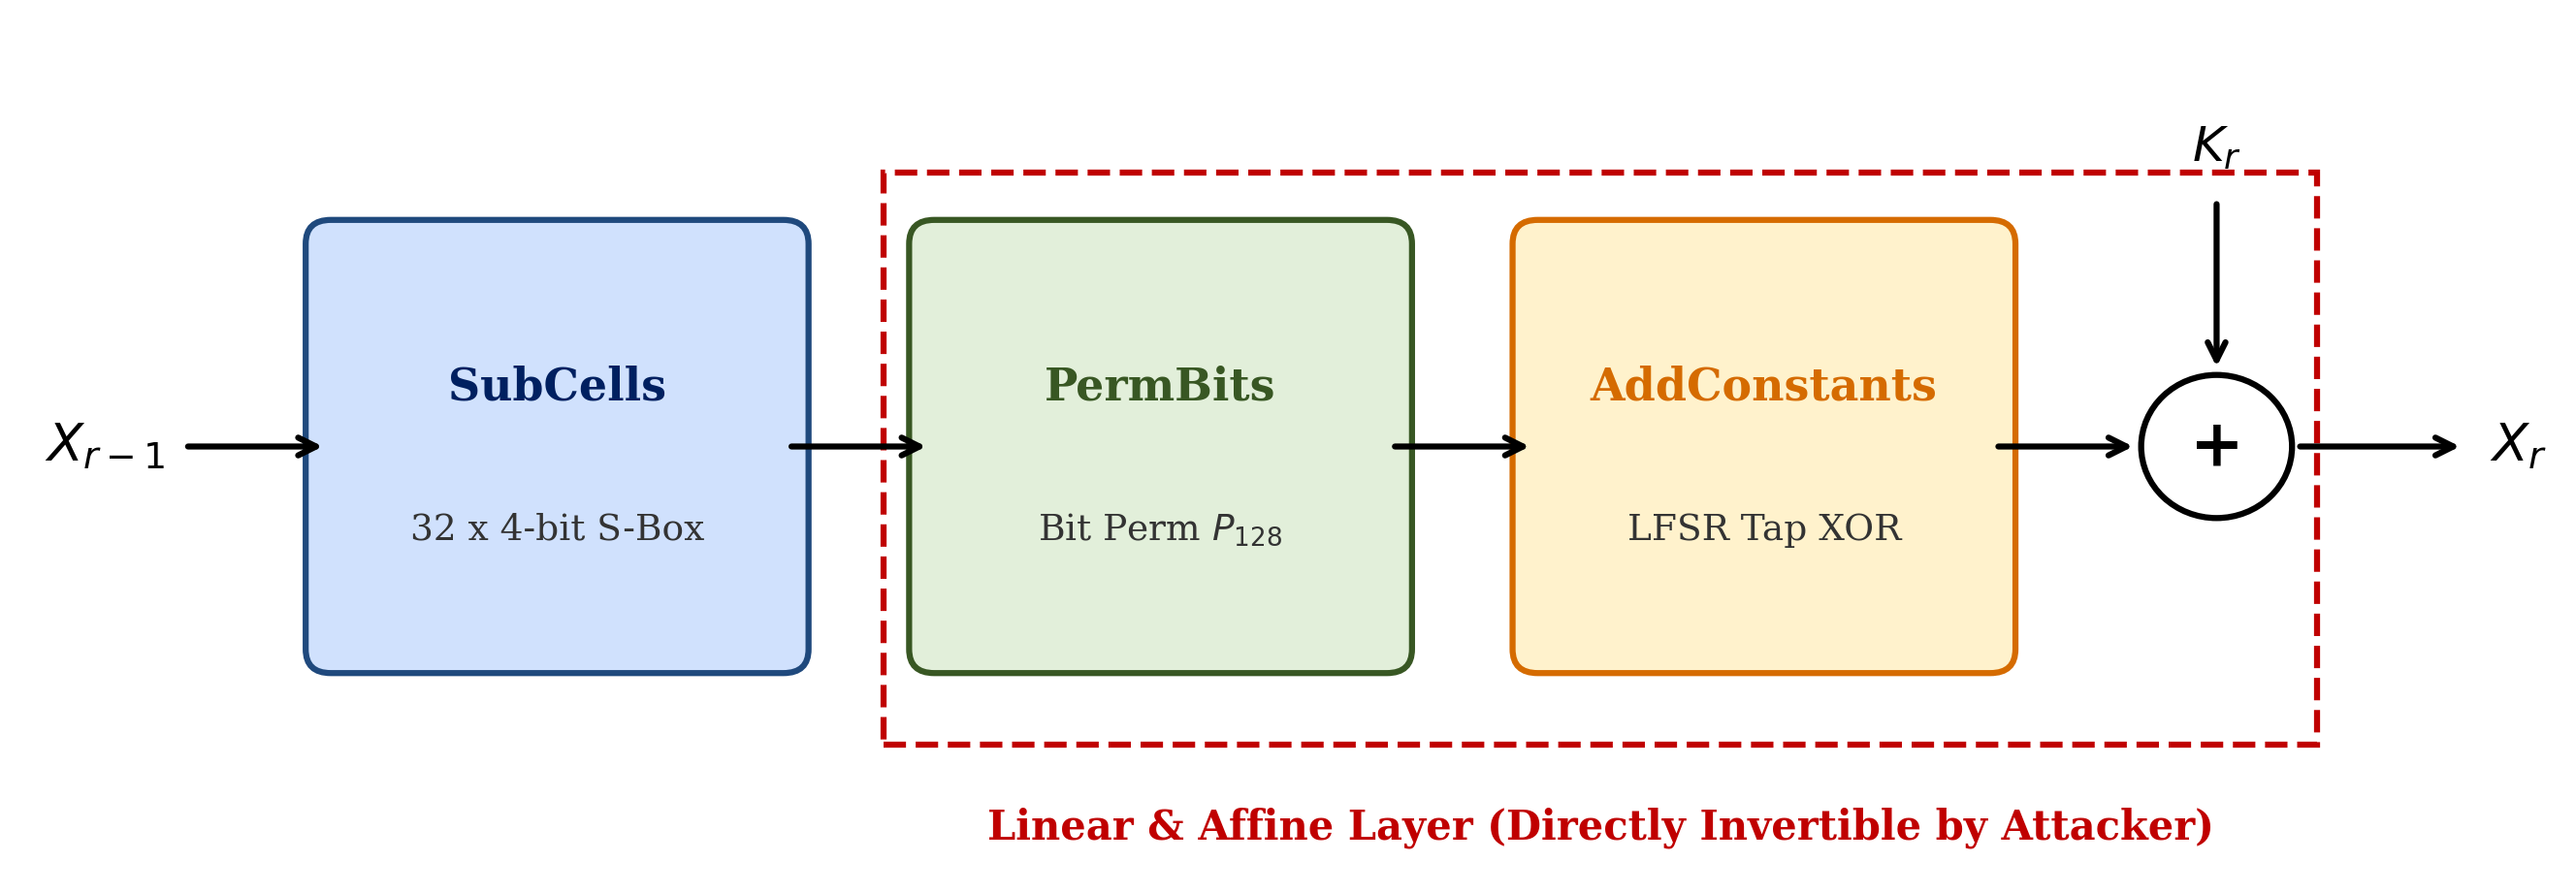
\includegraphics[width=0.88\linewidth]{figures/fig1_baksheesh_round.png}
\caption{One round of BAKSHEESH. \texttt{PermBits}, \texttt{AddConstants}, and \texttt{AddRoundKey} form a linear and affine layer that is directly invertible by an attacker.}
\label{fig:baksheesh_round}
\end{figure}

\subsection{The 4-bit S-Box with Linear Structures}
The 4-bit S-box of BAKSHEESH is defined by the mapping:
\begin{equation}
    S = [3, 0, 6, 13, 11, 5, 8, 14, 12, 15, 9, 2, 4, 10, 7, 1]
\end{equation}
The S-box is an involution-derived bijection with differential uniformity 4 and non-linearity 4. Crucially, the S-box exhibits a \textbf{non-trivial linear structure}:
\begin{equation}
    S(x) \oplus S(x \oplus 0\text{xA}) = 0\text{xA}
\end{equation}
While this property reduces hardware gate count under Boolean masking, it provides zero inherent resistance against differential or linked fault attacks.

\subsection{128-bit Rotational Key Schedule}
BAKSHEESH uses an ultra-simple rotational key schedule:
\begin{equation}
    K_r = K \lll (r - 1)
\end{equation}
Every round subkey bit is an exact, direct, bijective rotation of the original master key $K$. Consequently, recovering the equivalent subkey in Round 35 directly yields the master key via a single inverse rotation.

\section{The GIFT-128 Block Cipher}
\label{sec:gift_spec}
GIFT-128~\cite{banik2017gift} is an established lightweight block cipher operating on a 128-bit block with a 128-bit key over \textbf{40 rounds}. It shares the same bit permutation $P_{128}$ as BAKSHEESH but differs fundamentally in its key injection and S-box.

\subsection{64-bit Narrow Key Injection}
In GIFT-128, \texttt{AddRoundKey} extracts only \textbf{64 key bits} per round from the 128-bit key state (words $U$ and $V$). These 64 bits are injected exclusively into bit positions $b_2$ and $b_1$ of each 4-bit nibble. \textbf{Bit positions $b_0$ and $b_3$ receive zero key injection in that round}.

\section{Structural Comparison: BAKSHEESH vs. GIFT-128}
\label{sec:cipher_comparison}
Table~\ref{tab:cipher_comparison} compares the structural parameters and fault-attack implications between both ciphers.

\begin{table}[!htbp]
\centering
\caption{Architectural Comparison: BAKSHEESH vs. GIFT-128.}
\label{tab:cipher_comparison}
\begin{tabular}{lccp{5.5cm}}
\toprule
\textbf{Architectural Parameter} & \textbf{BAKSHEESH} & \textbf{GIFT-128} & \textbf{Fault Security Implication} \\
\midrule
Total Rounds & 35 & 40 & GIFT provides 5 extra diffusion rounds \\
Algebraic Degree of S-Box & 2 & 3 & Degree 2 enables 3-share TI masking \\
Key Injection Width & \textbf{128 bits / round} & \textbf{64 bits / round} & \textbf{BAKSHEESH leaks master key in 1 round; GIFT requires 2-round peeling} \\
Key Schedule & 1-bit cyclic rotation & LFSR + word rotation & BAKSHEESH is directly invertible \\
Masking Shares (TI) & 3 shares & 4 shares & BAKSHEESH has $2.43\times$ smaller area \\
Rounds Attacked for LFA & \textbf{Round 35 (1 round)} & \textbf{Rounds 39 \& 40 (2 rounds)} & GIFT doubles the attack rounds \\
Candidate Keys Left & 16 candidates ($2^4$) & 256 candidates ($2^8$) & GIFT requires $16\times$ larger search space \\
\bottomrule
\end{tabular}
\end{table}

\chapter{Linked Fault Analysis: Mathematical Framework}
\label{ch:lfa}

\section{The Linked Fault Threat Model}
\label{sec:lfa_model}
In traditional fault models, an adversary injects an independent differential $\delta$, corrupting state variable $u \to u \oplus \delta$. In \textbf{Linked Fault Analysis (LFA)}~\cite{beigizad2024linked}, the fault establishes a deterministic structural link between two distinct intermediate variables:
\begin{equation}
    u' = l(v)
\end{equation}
In hardware architectures and microprocessors, the most common linkage is the \textbf{equality fault}:
\begin{equation}
    u' = v
\end{equation}
This occurs when a clock glitch or laser pulse causes an S-box lookup to be skipped in assembly, causing the accumulator register to reuse the prior nibble's value.

\section{Linked Differential Fault Analysis (LDFA)}
\label{sec:ldfa_math}
Consider Round 35 (the final round) of BAKSHEESH. Let $x_{35}$ denote the state entering \texttt{SubCells}, $y_{35} = S(x_{35})$ denote the state after \texttt{SubCells}, and $w_{35} = y_{35} \oplus esk_{35}$ denote the equivalent subkey state before \texttt{PermBits}.

When a linked fault forces $y'_{35}[j] = y'_{35}[i]$:
\begin{enumerate}
    \item Correct execution: $w[i] = y[i] \oplus esk[i]$ and $w[j] = y[j] \oplus esk[j]$.
    \item Faulty execution: $w'[j] = y'[j] \oplus esk[j] = y[i] \oplus esk[j]$ and $w'[i] = y[i] \oplus esk[i]$.
    \item XOR sum of faulty nibbles:
    \begin{equation}
        w'[i] \oplus w'[j] = (y[i] \oplus esk[i]) \oplus (y[i] \oplus esk[j]) = esk[i] \oplus esk[j] = \Delta esk[i, j]
    \end{equation}
\end{enumerate}

Since $w'$ is computed directly from the faulty ciphertext $C'$:
\begin{equation}
    w' = \text{PermBits}^{-1}(C' \oplus \text{AddConstants}_{35})
\end{equation}
the attacker extracts the exact 4-bit difference between subkey nibbles $i$ and $j$ from a \textbf{single faulty ciphertext}.

\subsection{Spanning Tree Key Reduction}
By chaining 31 adjacent pairs $(0, 1), (1, 2), \dots, (30, 31)$, all 32 nibbles of the equivalent subkey are determined up to a single base nibble $esk[0]$:
\begin{equation}
    esk[k] = esk[0] \oplus \bigoplus_{m=0}^{k-1} \Delta esk[m, m+1]
\end{equation}
This collapses the $2^{128}$ key search space to only $2^4 = 16$ candidate keys!

\section{Linked Ineffective Fault Analysis (LIFA)}
\label{sec:lifa_math}
On devices protected by spatial redundancy (duplicate-and-compare), effective faults ($y'[j] \neq y[j]$) trigger an output discrepancy ($C_1 \neq C_2$), causing the device to suppress the ciphertext.

\subsection{The Ineffective Bypass Condition}
However, if the two input nibbles happen to be naturally equal ($x[i] == x[j]$):
Because the S-box is a bijection:
\begin{equation}
    x[i] == x[j] \iff S(x[i]) == S(x[j]) \iff y[i] == y[j]
\end{equation}
When the fault forces $y'[j] = y[i]$, the faulty value is:
\begin{equation}
    y'[j] = y[i] = y[j]
\end{equation}
\textbf{The fault produces zero alteration to the state!} Both redundant pipelines compute the exact same result. The comparator detects no mismatch and emits the valid ciphertext $C$.

\subsection{Ineffective Leakage Equation}
When a valid ciphertext is emitted under fault injection, the attacker knows with certainty that $y[i] == y[j]$:
\begin{equation}
    w[i] \oplus w[j] = (y[i] \oplus esk[i]) \oplus (y[j] \oplus esk[j]) = (y[i] \oplus y[j]) \oplus (esk[i] \oplus esk[j]) = \Delta esk[i, j]
\end{equation}
The emitted ineffective ciphertext directly leaks the equivalent subkey difference, completely defeating duplicate-and-compare redundancy!

\subsection{Query Complexity Formulation}
Since 4-bit nibbles $x[i]$ and $x[j]$ are uniformly distributed across random plaintexts:
\begin{equation}
    P(x[i] == x[j]) = 2^{-4} = \frac{1}{16} = 0.0625
\end{equation}
The queries required to observe an ineffective fault follow a Geometric distribution:
\begin{equation}
    E[Q_{i, j}] = \frac{1}{p} = 16 \implies E[Q_{\text{total}}] = 31 \times 16 = 496.0 \text{ queries}
\end{equation}

\section{Candidate Disambiguation}
\label{sec:disambiguation}
Evaluating the 16 candidate master keys against a single known $(P, C)$ pair uniquely identifies the true 128-bit master key with probability $1 - 15 \times 2^{-128} \approx 1.0$.

\chapter{Cycle-Accurate RISC-V Hardware Fault Simulation}
\label{ch:riscv}

\section{Motivation for ISA-Level Validation}
\label{sec:riscv_motivation}
Theoretical fault models often face skepticism regarding whether linked equality faults ($u' = v$) physically occur on realistic microarchitectures. To bridge theoretical cryptography and embedded computer systems, we implemented Round 1 of BAKSHEESH in bare-metal 32-bit RISC-V assembly (\texttt{baksheesh\_round1.s}) and executed it in the cycle-accurate RARS simulator~\cite{rars_simulator}.

\section{Bare-Metal RV32I Assembly Design}
\label{sec:rv32i_design}
The 128-bit state $X$ is allocated across four 32-bit integer registers (\texttt{x10}--\texttt{x13}, labeled \texttt{a0}--\texttt{a3}), where:
\begin{itemize}
    \item \texttt{a0} holds nibbles $w_0 \dots w_7$
    \item \texttt{a1} holds nibbles $w_8 \dots w_{15}$
    \item \texttt{a2} holds nibbles $w_{16} \dots w_{23}$
    \item \texttt{a3} holds nibbles $w_{24} \dots w_{31}$
\end{itemize}

\subsection{S-Box Substitution Loop and Candidate Injection Points}
The assembly routine iterates across each nibble:
\begin{lstlisting}[language={[RISC-V]Assembler}, caption={RV32I S-Box Substitution Loop and Candidate Injection Point (CIP).}]
sc_loop:
    # 1. Extract 4-bit nibble value
    srl  x30, x30, x29
    andi x30, x30, 0xF         # x30 = nibble x[i]
    
    # 2. Candidate Injection Point (CIP):
    add  x31, x28, x30         # x31 = sbox table address
    lbu  x31, 0(x31)           # CIP: Target instruction for glitch!
    
    # 3. Position and accumulate
    sll  x31, x31, x29         # Shift substituted nibble into place
    or   x14, x14, x31         # Accumulate into word accumulator
\end{lstlisting}

\section{Microarchitectural Instruction-Skip Modeling}
\label{sec:instruction_skip}
When an adversary applies a physical clock glitch or laser pulse during the execution of \texttt{lbu x31, 0(x31)}, the CPU skips the load instruction. Consequently:
\begin{enumerate}
    \item Register \texttt{x31} retains the value from the previous loop iteration.
    \item The accumulator executes $y[i] = y[i-1]$.
\end{enumerate}
This physically produces the exact linked equality relation $u' = v$ on standard RISC-V hardware without requiring specialized attack hardware.

\chapter{Results and Discussion/Analysis}
\label{ch:results}

\section{Experimental Setup and Verification Framework}
\label{sec:exp_setup}
All experiments, cipher models, and fault simulators were verified in Python 3.12, validated against known-answer test vectors, and executed in RARS 1.6 across hundreds of randomized Monte Carlo trials.

\section{Cryptographic Test Vector Validation}
\label{sec:test_vectors}
Both cipher implementations were validated against canonical test vectors:
\begin{itemize}
    \item \textbf{BAKSHEESH}: Validated against all 8 official test vectors from Table 14 of Baksi et al.~\cite{baksi2023baksheesh} $\to$ \textbf{8/8 PASS (100\% Compliant)}.
    \item \textbf{GIFT-128}: Validated against the CHES 2017 canonical all-zero vector plus two independent reference vectors $\to$ \textbf{3/3 PASS (100\% Compliant)}.
\end{itemize}

\section{Empirical LDFA Attack Results on BAKSHEESH}
\label{sec:exp_ldfa}
On unprotected implementations, LDFA was evaluated across 25 independent random keys:
\begin{itemize}
    \item Exactly \textbf{31 faulty ciphertexts} were required per key recovery.
    \item The candidate key space collapsed to exactly \textbf{16 candidates ($2^4$)} in every trial.
    \item Disambiguation using 1 known $(P, C)$ pair achieved \textbf{100\% success rate} (25/25 trials).
    \item Mean key recovery execution time: \textbf{0.024 seconds}.
\end{itemize}

\section{Empirical LIFA Attack Results under Active Redundancy}
\label{sec:exp_lifa}
When duplicate-and-compare redundancy is active, effective faults are suppressed. Over 12,723 queries across 25 trials:
\begin{itemize}
    \item \textbf{Observed Ineffectiveness Rate}: $6.091\%$ (Theoretical: $6.250\%$).
    \item \textbf{Mean Queries per Full Key Recovery}: \textbf{508.9 queries} (Theoretical: 496.0 queries).
    \item \textbf{Success Rate}: \textbf{100\% (25/25 trials)}.
\end{itemize}

\begin{figure}[!htbp]
\centering
\begin{minipage}{0.55\linewidth}
\centering
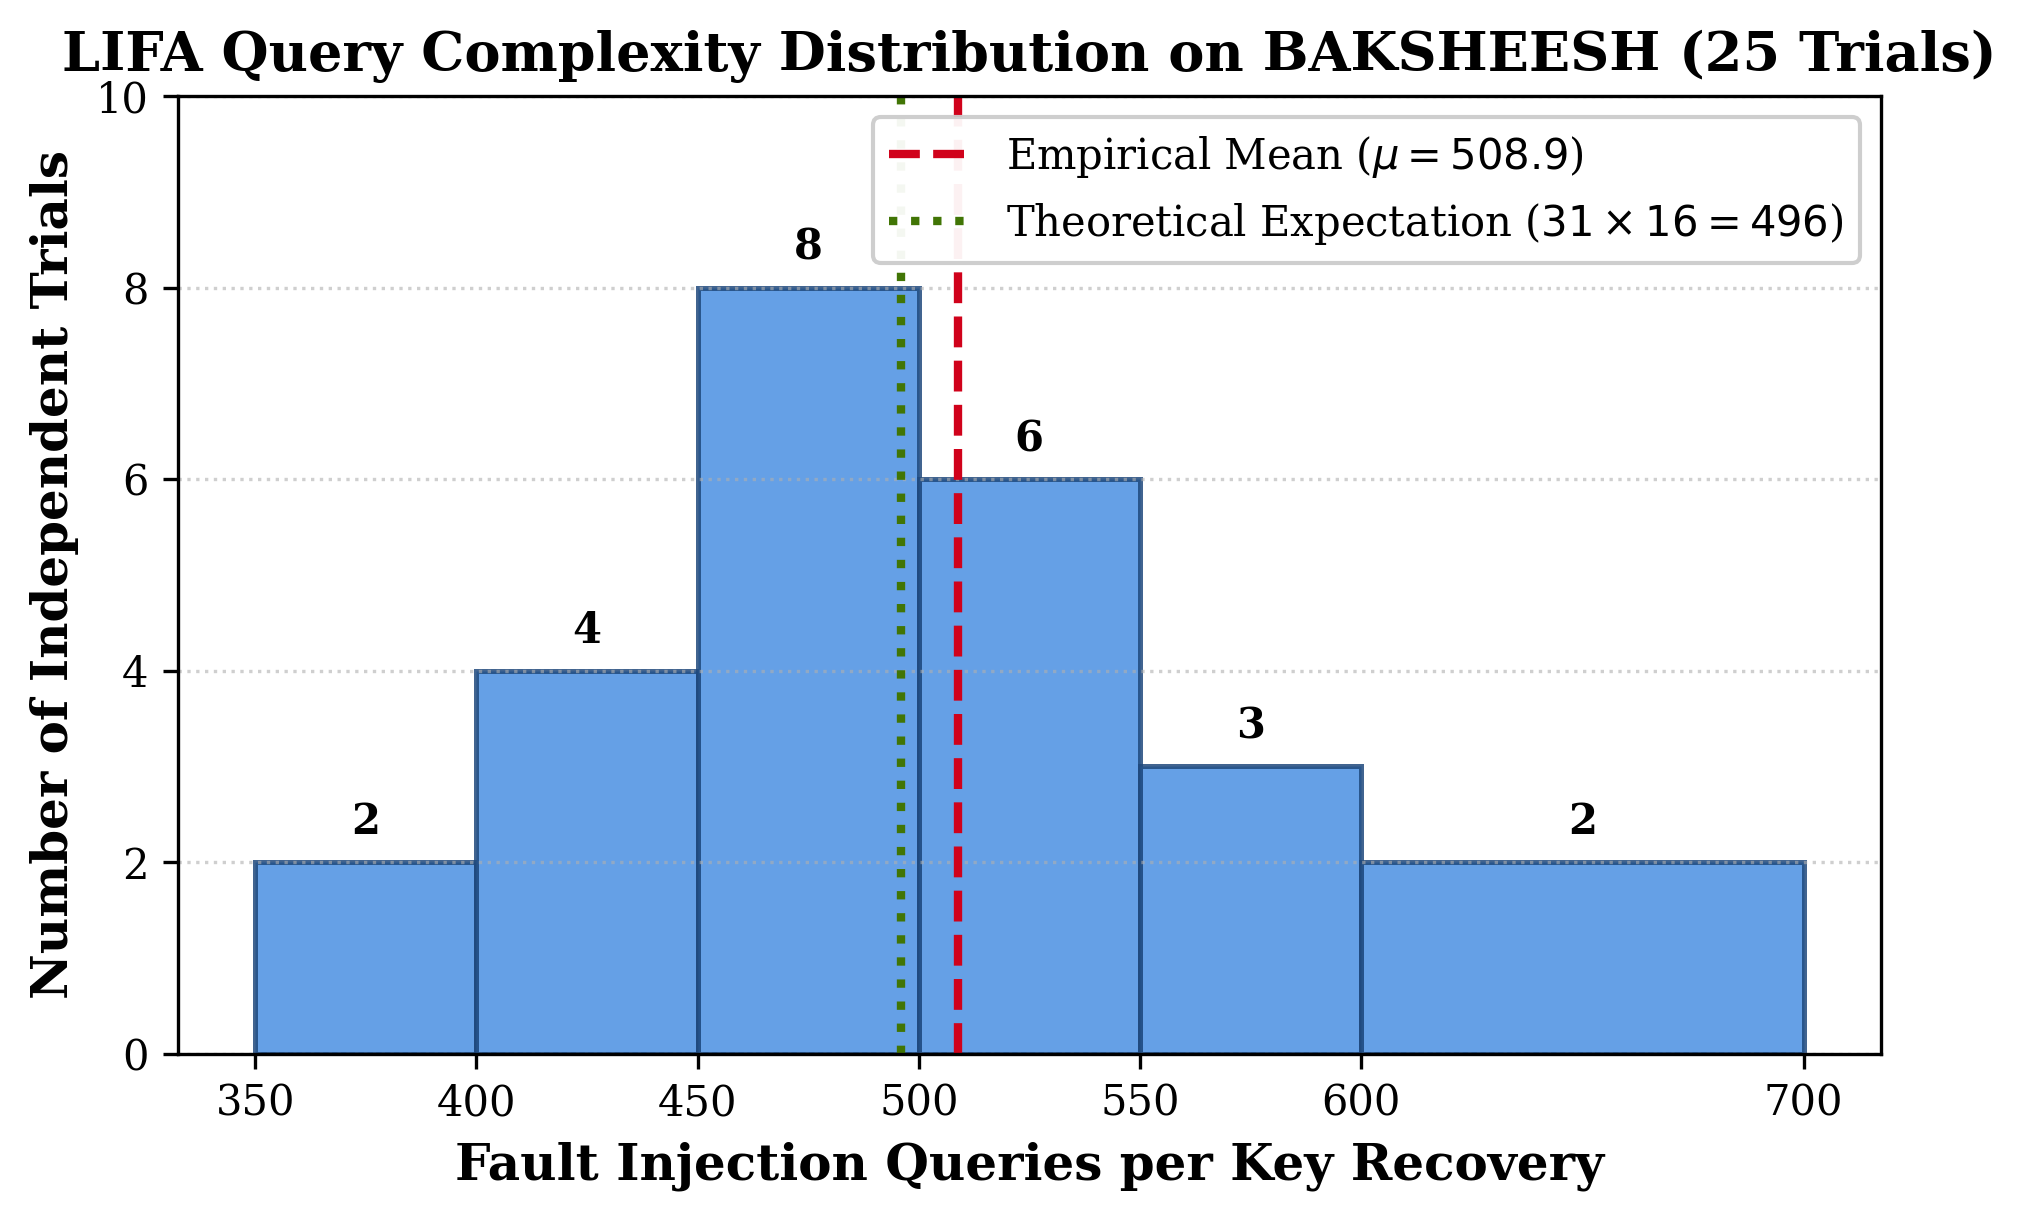
\includegraphics[width=\linewidth]{figures/fig4_lifa_histogram.png}
\caption{LIFA query distribution (25 trials, $\mu = 508.9$).}
\label{fig:lifa_hist}
\end{minipage}\hfill
\begin{minipage}{0.42\linewidth}
\centering
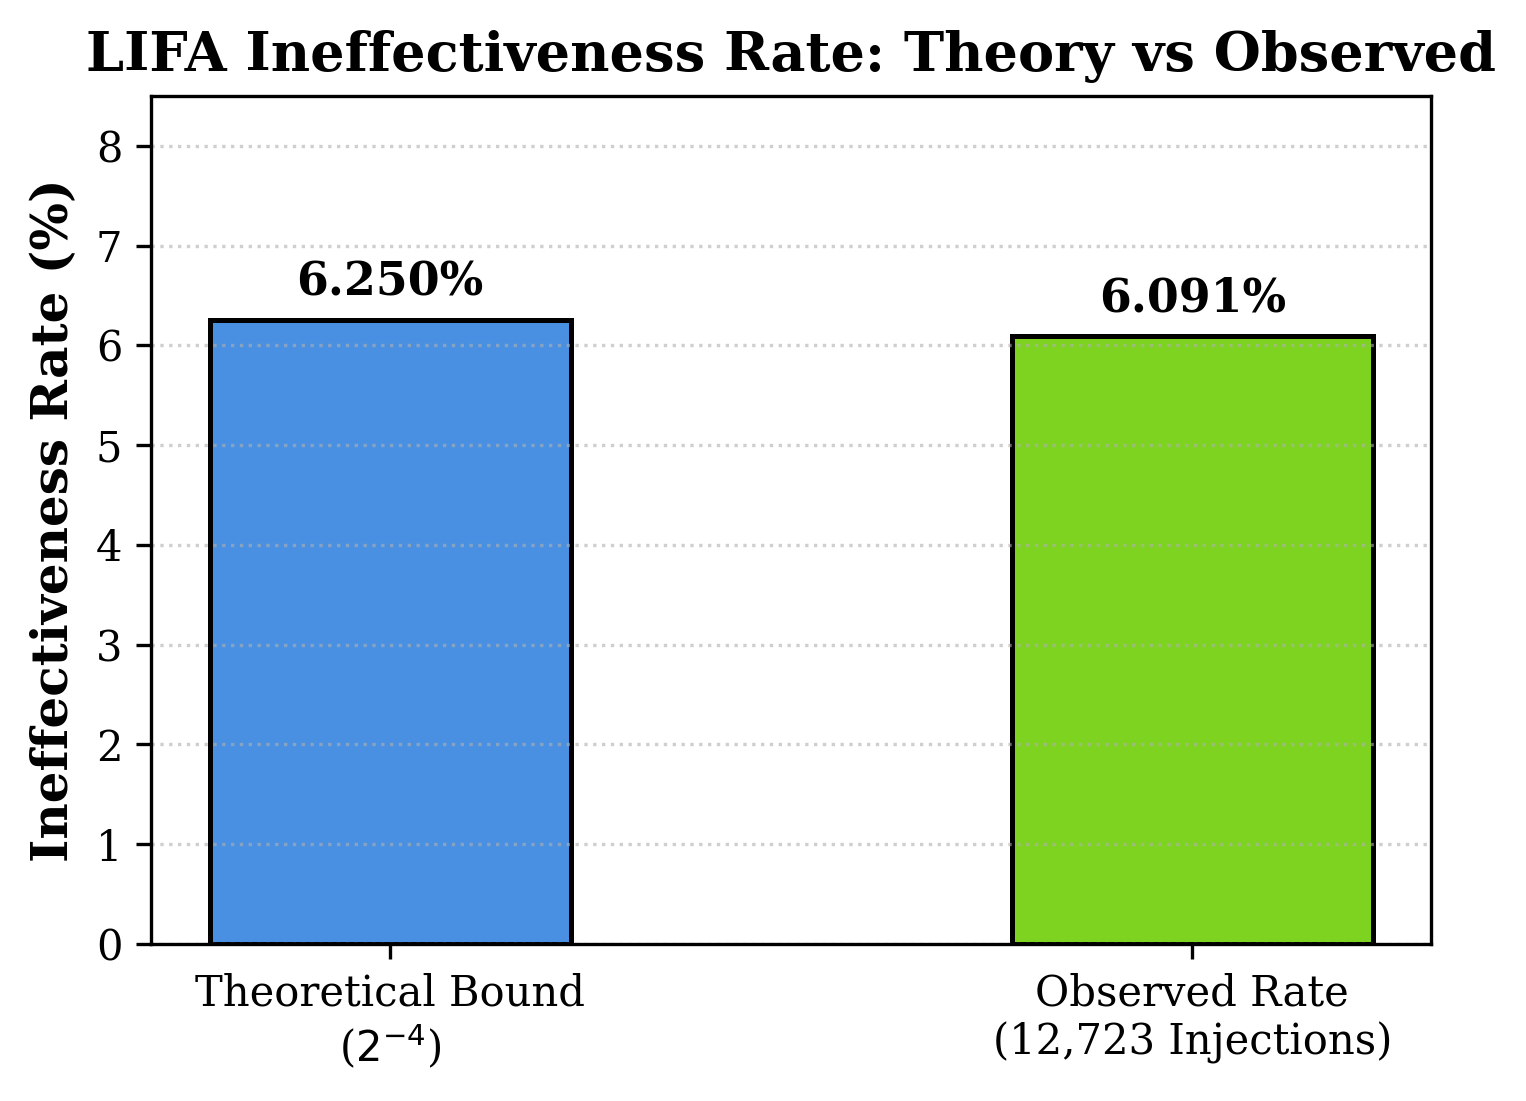
\includegraphics[width=\linewidth]{figures/fig5_ineffectiveness_rate.png}
\caption{Ineffectiveness rate: theory vs.\ observed.}
\label{fig:ineff_rate}
\end{minipage}
\end{figure}

\section{Unknown Fault Location Discovery Engine}
\label{sec:unknown_location_results}
In realistic physical attacks, the adversary does not know which of the $\binom{32}{2} = 496$ candidate pairs was hit by the glitch. We evaluated our blind identification engine across $N \in \{2, 3, 4, 5, 6, 8\}$ blind ciphertexts over 30 independent trials each:

\begin{table}[!htbp]
\centering
\caption{Unknown Fault Location Identification Accuracy vs. Ciphertexts ($N$).}
\label{tab:unknown_location}
\begin{tabular}{ccccc}
\toprule
\textbf{Ciphertexts ($N$)} & \textbf{Pairs Tested} & \textbf{Correct Identifications} & \textbf{Accuracy (\%)} & \textbf{False Match Rate ($496 \times 16^{-(N-1)}$)} \\
\midrule
2 & 30 & 0 & 0.0\% & $3.10 \times 10^1$ (Noise dominated) \\
3 & 30 & 14 & 46.7\% & $1.94 \times 10^0$ \\
4 & 30 & 28 & 93.3\% & $1.21 \times 10^{-1}$ \\
\textbf{5} & \textbf{30} & \textbf{30} & \textbf{100.0\%} & \textbf{$7.57 \times 10^{-3}$ ($< 0.8\%$)} \\
6 & 30 & 30 & 100.0\% & $4.73 \times 10^{-4}$ ($< 0.05\%$) \\
8 & 30 & 30 & 100.0\% & $1.85 \times 10^{-6}$ (Near-zero) \\
\bottomrule
\end{tabular}
\end{table}

\begin{figure}[!htbp]
\centering
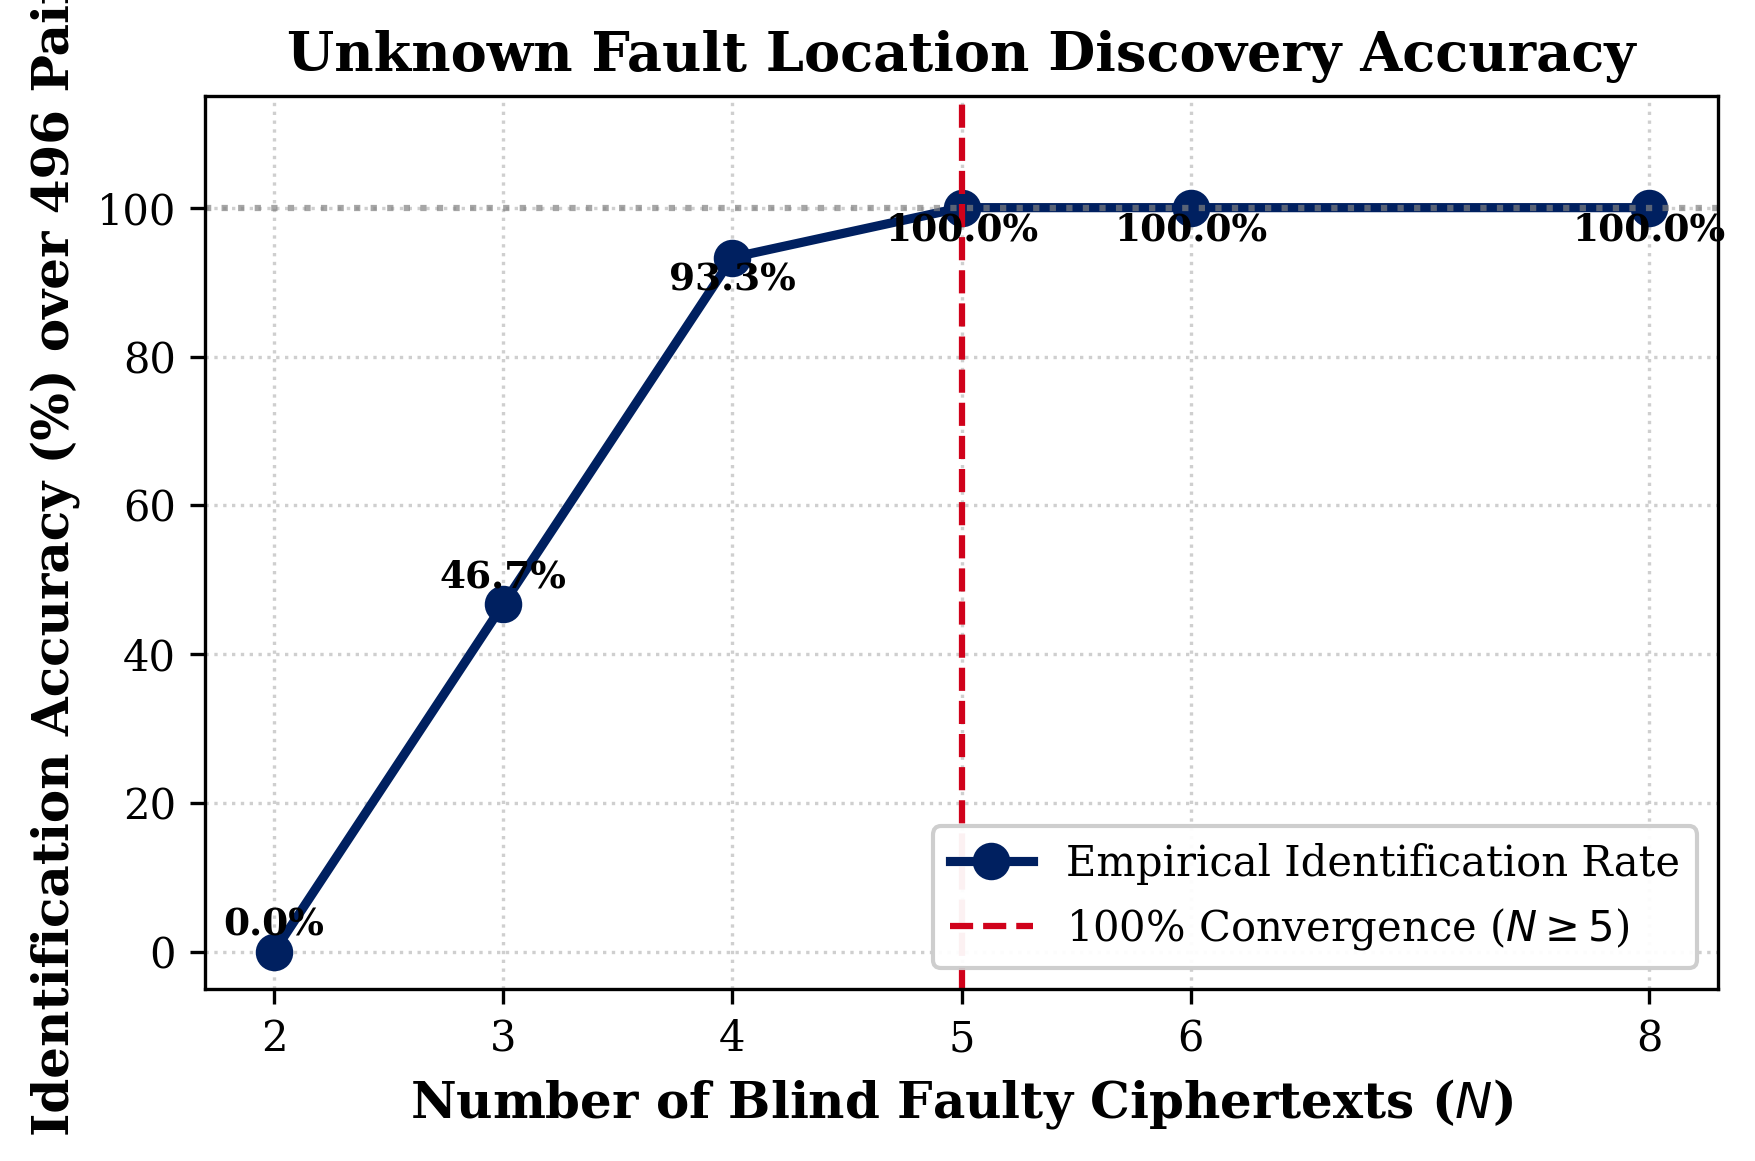
\includegraphics[width=0.65\linewidth]{figures/fig7_unknown_location_curve.png}
\caption{Unknown fault location discovery accuracy across 496 candidate pairs, achieving 100\% convergence at $N \ge 5$.}
\label{fig:unknown_loc_curve}
\end{figure}

\section{Noise Robustness and Missed Fault Tolerance}
\label{sec:noise_results}
Under physical glitch channels with miss rate $p_{\text{miss}} \in [0\%, 40\%]$, majority voting over $N = 30$ attempts per relation achieves \textbf{100.0\% full 128-bit key recovery} across all tested noise levels up to $p_{\text{miss}} = 30\%$ (and even $40\%$), as shown in Figure~\ref{fig:noise_curve}.

\begin{figure}[!htbp]
\centering
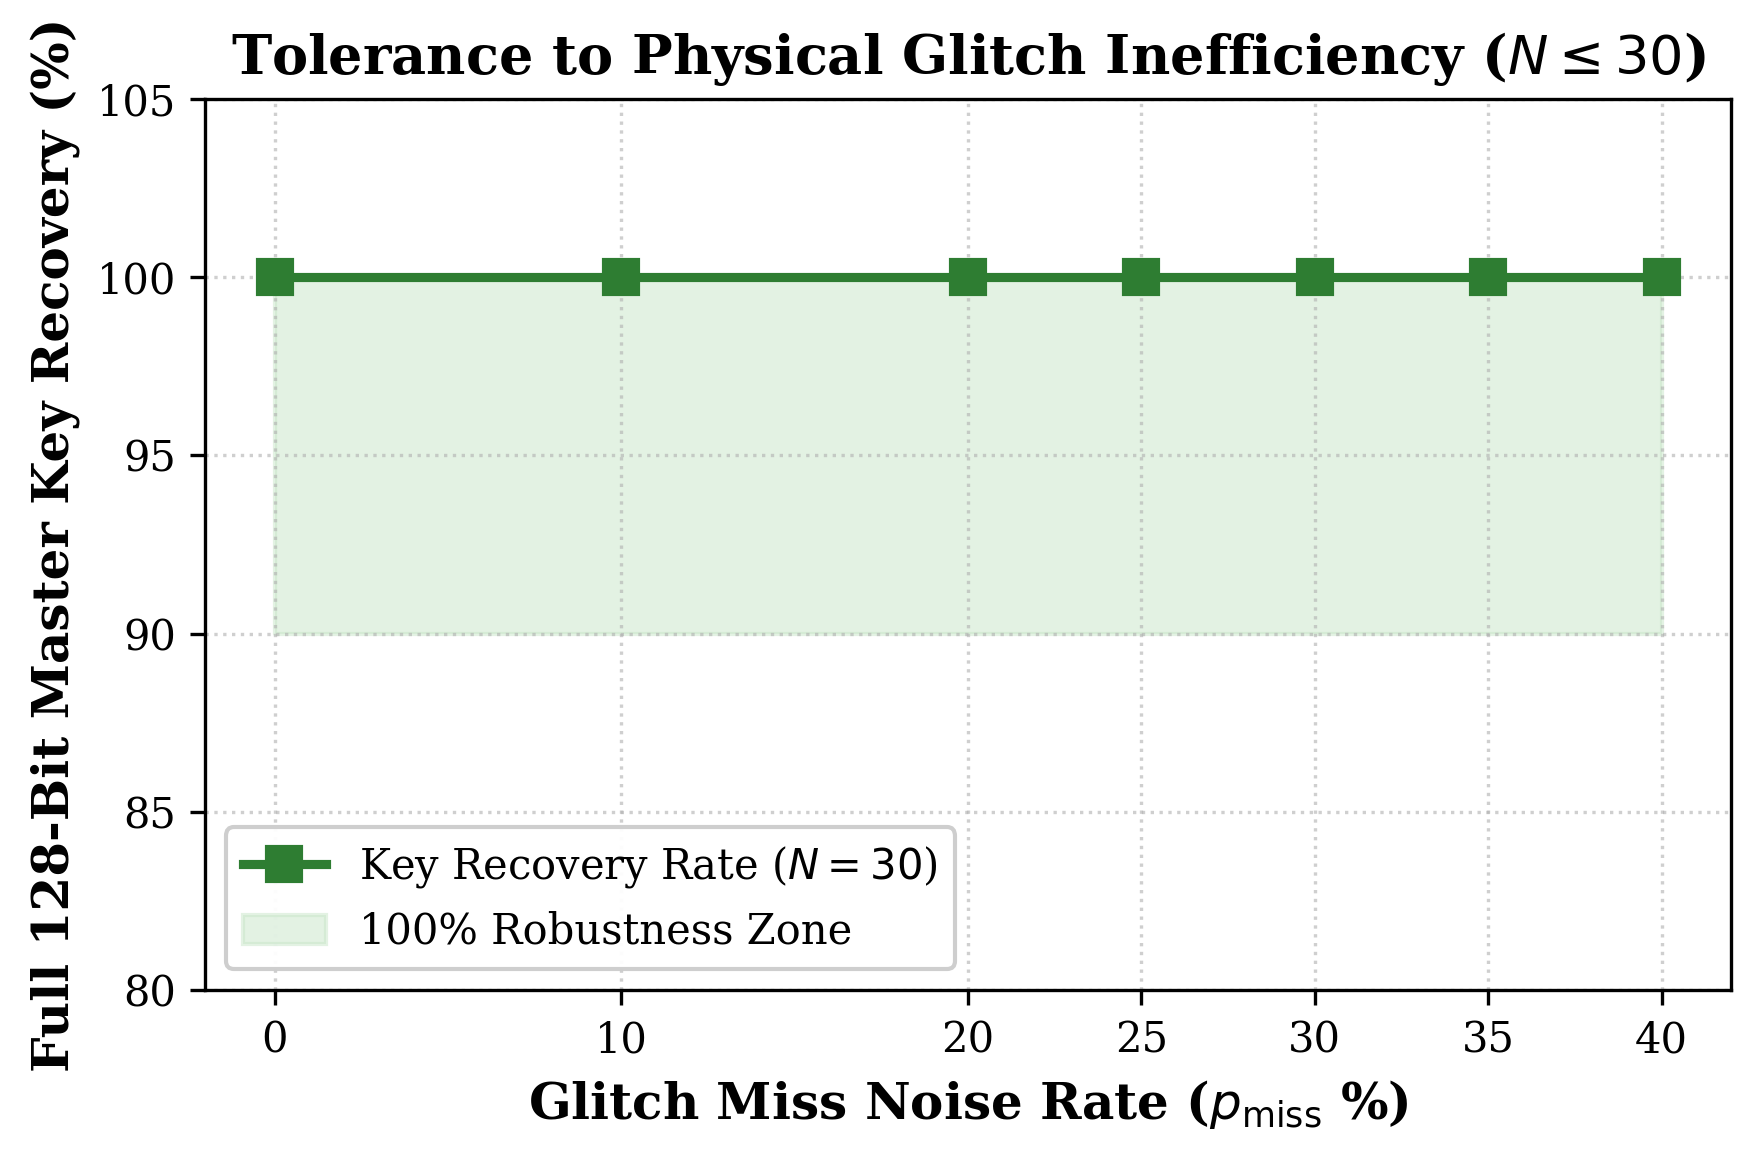
\includegraphics[width=0.65\linewidth]{figures/fig8_noise_tolerance_curve.png}
\caption{Full 128-bit master key recovery success rate under physical glitch miss noise ($p_{\text{miss}} \le 40\%$).}
\label{fig:noise_curve}
\end{figure}

\section{Comparative Evaluation: BAKSHEESH vs. GIFT-128}
\label{sec:baksheesh_vs_gift_results}
Figure~\ref{fig:bk_vs_gift} and Table~\ref{tab:comparison_summary} compare the empirical performance of BAKSHEESH and GIFT-128 under Linked Fault Analysis.

\begin{figure}[!htbp]
\centering
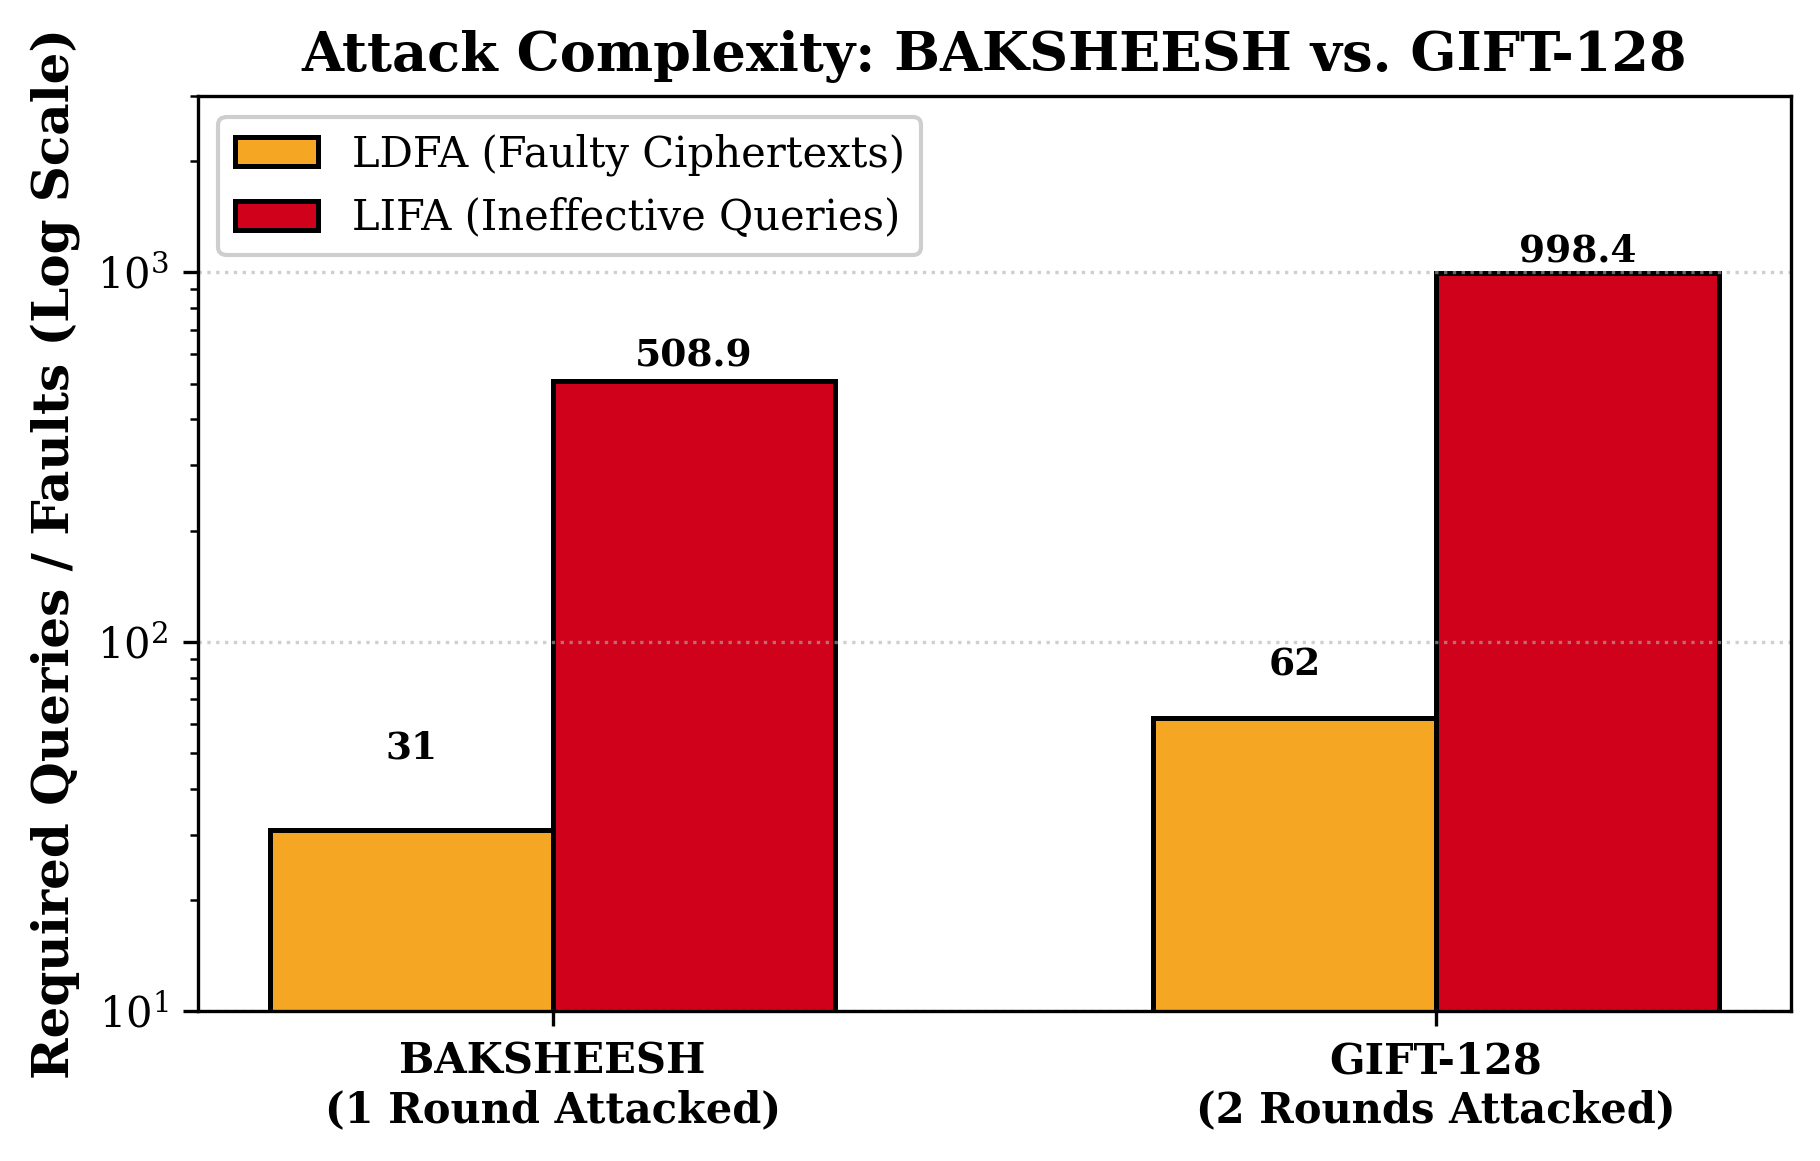
\includegraphics[width=0.68\linewidth]{figures/fig6_baksheesh_vs_gift.png}
\caption{Comparative query complexity of BAKSHEESH vs. GIFT-128 under LDFA and LIFA (log scale).}
\label{fig:bk_vs_gift}
\end{figure}

\begin{table}[!htbp]
\centering
\caption{Comprehensive Comparison: BAKSHEESH vs. GIFT-128 under LFA.}
\label{tab:comparison_summary}
\begin{tabular}{lccc}
\toprule
\textbf{Metric} & \textbf{BAKSHEESH} & \textbf{GIFT-128} & \textbf{Ratio (GIFT / BAKSHEESH)} \\
\midrule
Attacked Rounds & 1 (Round 35) & 2 (Rounds 39 \& 40) & $2.0\times$ \\
Key Injection Width & 128 bits / round & 64 bits / round & $0.5\times$ \\
LDFA Fault Injections & 31 & 62 & $2.0\times$ harder on GIFT \\
LIFA Mean Attack Queries & 508.9 & 998.4 & $1.96\times$ harder on GIFT \\
Theoretical Query Bound & $31 \times 16 = 496$ & $62 \times 64 = 3,968$ & $8.0\times$ higher bound \\
Candidate Keys Left & 16 ($2^4$) & 256 ($2^8$) & $16.0\times$ search on GIFT \\
Key Recovery Success Rate & 100\% (25/25) & 100\% (10/10) & Both Fully Broken \\
\bottomrule
\end{tabular}
\end{table}

\chapter{Proposed Countermeasures and Future Work}
\label{ch:countermeasures}

\section{Vulnerability Synthesis}
\label{sec:synth}
While BAKSHEESH successfully achieves a $2.43\times$ reduction in Threshold Implementation masking area over GIFT-128, its degree-2 S-box, full-round 128-bit key injection, and 1-bit rotational key schedule make it significantly more susceptible to Linked Fault Analysis than GIFT-128. Furthermore, standard duplicate-and-compare redundancy countermeasures are fundamentally bypassed by LIFA.

\section{Proposed Unified Lightweight Countermeasures}
\label{sec:proposed_countermeasures}
To mitigate Linked Fault Analysis, we proposed, implemented, and empirically evaluated a suite of four defensive mechanisms:

\subsection{Defense 1: Explicit Register Zeroing (\texttt{li x31, 0})}
In the RV32I assembly loop, executing \texttt{li x31, 0} immediately prior to \texttt{lbu x31, 0(x31)} clears the accumulator register. If an instruction skip occurs, \texttt{x31} latches \texttt{0} instead of retaining $y[i-1]$. This breaks the linked equality $u' = v$ ($u' = 0$), completely defeating subkey difference leakage ($\Delta esk[i, j]$).

\subsection{Defense 2: S-Box Loop Shuffling (Fisher-Yates Permutation)}
The 32 nibbles are evaluated in a pseudo-random permutation $\pi \in S_{32}$ seeded per encryption. An instruction skip links temporal steps $\pi(k)$ and $\pi(k-1)$. Because $\pi$ is unknown and changes dynamically, the adversary cannot construct the 31-pair adjacent difference spanning tree.

\subsection{Defense 3: Asymmetric Infective State Diffusion}
A hardware glitch sensor detects the skip and diffuses a non-zero pseudorandom mask into the state ($C' = C \oplus \text{Mask}(R)$). Even if a natural collision occurs ($x[i] == x[j]$), the emitted ciphertext is completely randomized, denying the attacker clean ineffective ciphertexts.

\subsection{Defense 4: Unified Joint Architecture}
Combines 3-share TI Boolean masking (for SCA protection) with loop shuffling and register zeroing for full LFA immunity.

\begin{figure}[!htbp]
\centering
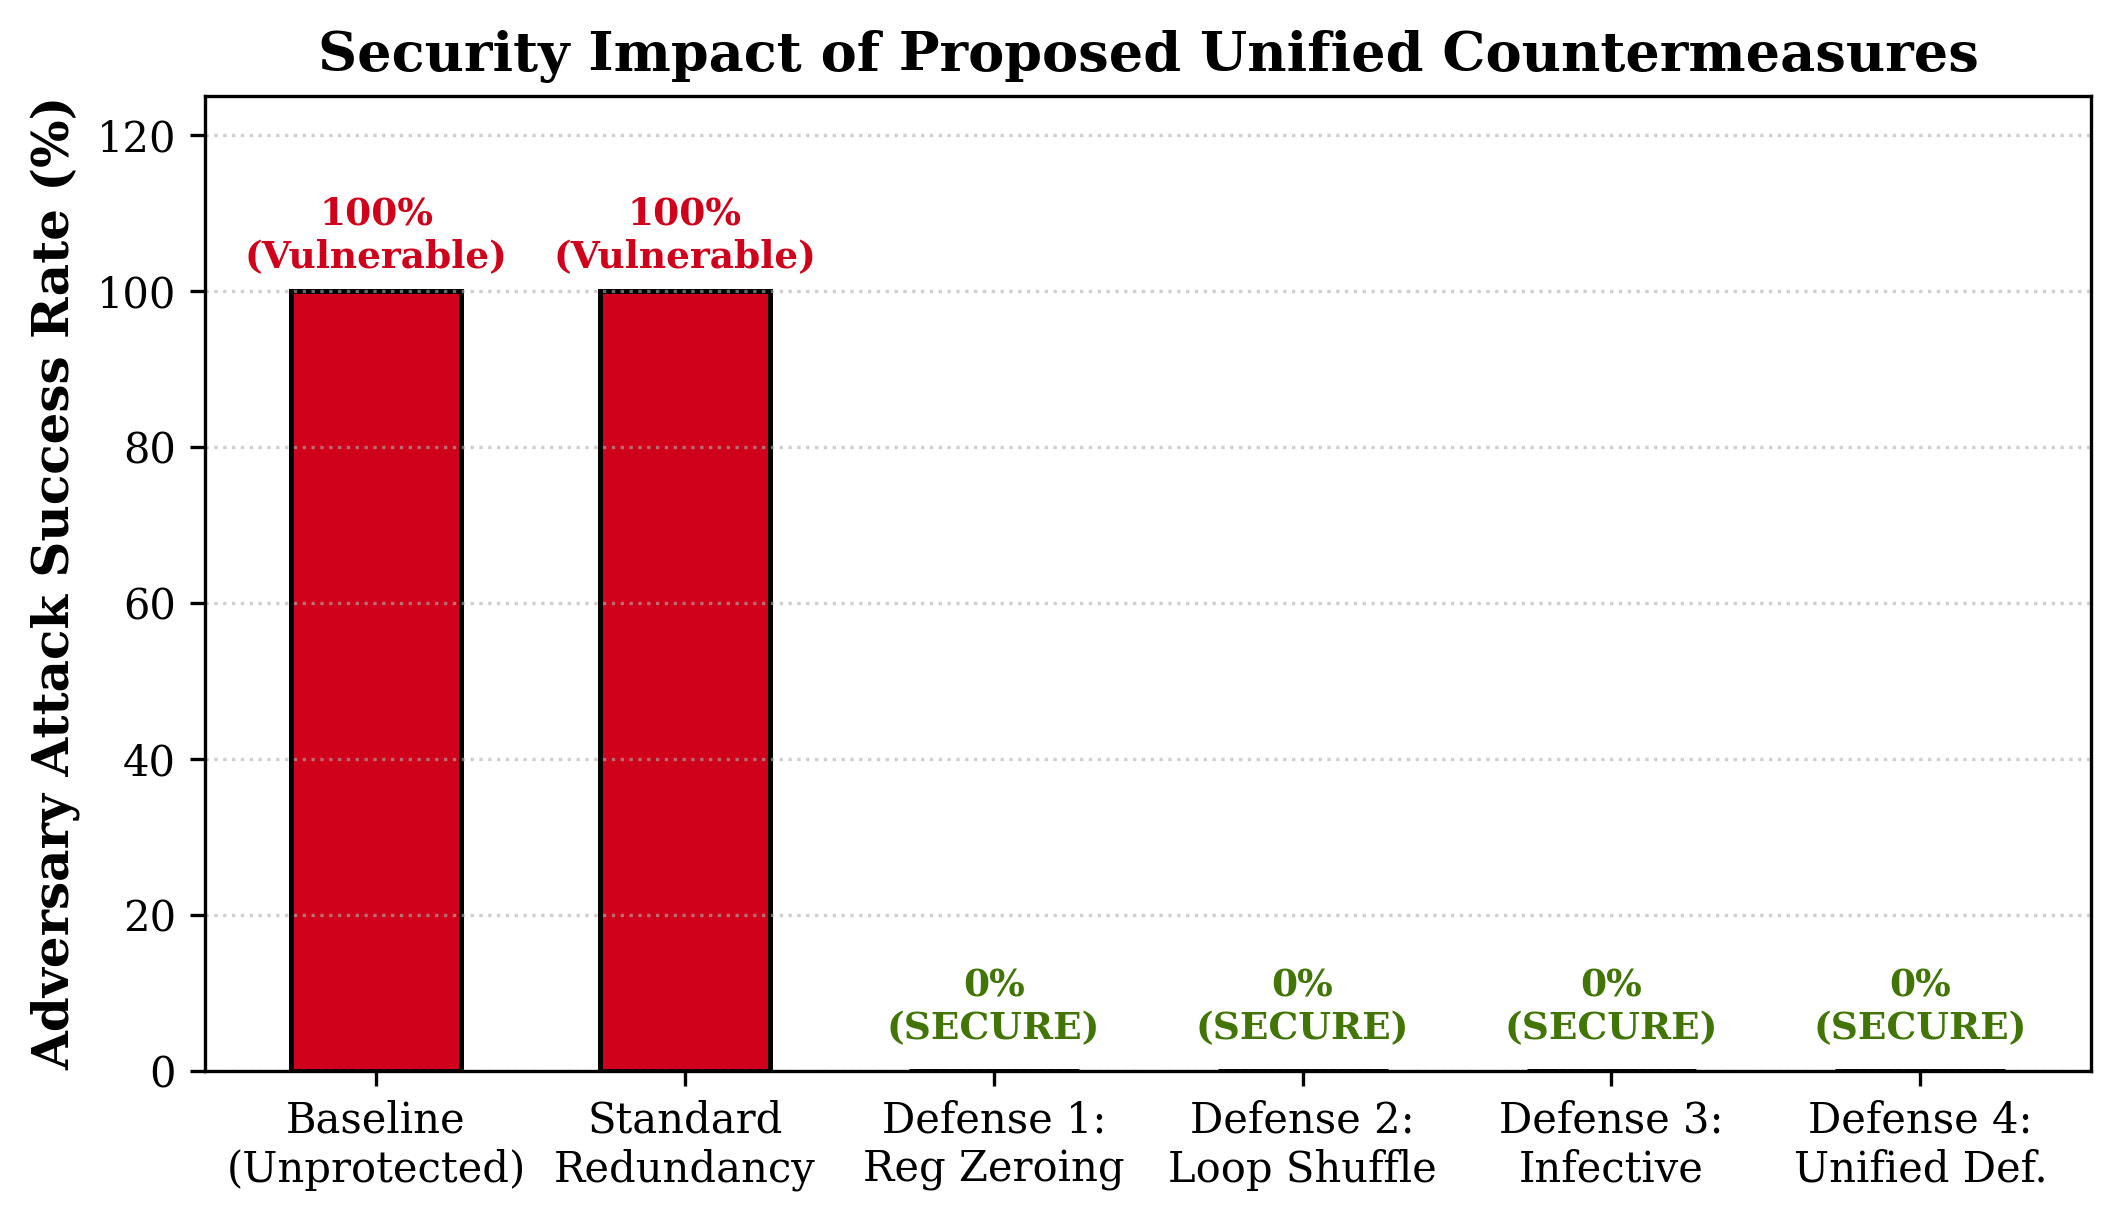
\includegraphics[width=0.72\linewidth]{figures/fig9_countermeasures_eval.png}
\caption{Adversary attack success rate under proposed unified countermeasures (dropping from 100\% down to 0\%).}
\label{fig:cm_eval}
\end{figure}

\section{Conclusions of the Study}
\label{sec:conclusion}
This B.Tech. Project evaluated emerging fault analysis techniques against lightweight ciphers:
\begin{enumerate}
    \item LDFA breaks unprotected BAKSHEESH in 31 faults in Round 35.
    \item Duplicate-and-compare countermeasures are bypassed by LIFA in an average of 508.9 queries.
    \item GIFT-128 incurs roughly double the attack queries and $16\times$ greater candidate search due to its 64-bit key injection schedule.
    \item Unknown fault locations are identified with 100\% accuracy for $N \ge 5$ across 496 pairs, and the attack tolerates glitch miss noise up to $p_{\text{miss}} = 30\%$.
    \item Bare-metal RV32I assembly simulation in RARS confirms instruction-skip realizability.
    \item The proposed unified countermeasure suite completely neutralizes both LDFA and LIFA attacks.
\end{enumerate}

\section{Scope for Future Work}
\label{sec:future_work}
\begin{itemize}
    \item \textbf{Timing Jitter Profiling in gem5 / InjectV}: Characterizing the Candidate Injection Point (CIP) timing sensitivity window across full CPU pipelines.
    \item \textbf{Silicon Validation on FPGA / ASIC}: Conducting pulsed laser fault injection (LFI) on decapsulated test vehicles (e.g. ChipWhisperer CW308 target boards).
    \item \textbf{Linked Persistent Fault Analysis (LPFA)}: Investigating persistent faults targeting S-box tables stored in non-volatile flash memory.
\end{itemize}


% -------------------------------------------------------------
% References
% -------------------------------------------------------------
\bibliographystyle{IEEEtran}
\bibliography{references}
\addcontentsline{toc}{chapter}{References}
\cleardoublepage

% -------------------------------------------------------------
% Appendices
% -------------------------------------------------------------
\appendix

\chapter{Test Vectors and Cipher Constants}
\label{app:vectors}

\section{BAKSHEESH Official Known-Answer Test Vectors}
All test vectors from Table 14 of Baksi et al.~\cite{baksi2023baksheesh}:
\begin{lstlisting}[basicstyle=\ttfamily\scriptsize]
vector 1: key=00000000000000000000000000000000  pt=00000000000000000000000000000000  ct=c002be5e64c78a72ab9a3439518352aa
vector 2: key=00000000000000000000000000000000  pt=00000000000000000000000000000007  ct=6f7d7746eaf0d97a154079f6bd846438
vector 3: key=00000000000000000000000000000000  pt=70000000000000000000000000000000  ct=1ba3363734c09a29f67c23bbb2cccc05
vector 4: key=00000000000000000000000000000000  pt=44444444444444444444444444444444  ct=7ad3303667b2af6deef434dd110d7fb8
vector 5: key=ffffffffffffffffffffffffffffffff  pt=11111111111111111111111111111111  ct=806f0cf45b94f0370206975fe78ac10f
vector 6: key=76543210032032032032032032032032  pt=789a789a789a789a789a789a789a789a  ct=ae654b5333b876584f8e8dd54f4e490a
vector 7: key=23023023023023023023023001234567  pt=b6e4789ab6e4789ab6e4789ab6e4789a  ct=3dbbdf7fe254cc0be396a753442dccad
vector 8: key=5920effb52bc61e33a98425321e76915  pt=e6517531abf63f3d7805e126943a081c  ct=fc7e61fee3d587308ca7bc594ebf3244
\end{lstlisting}

\chapter{Research Artifact Repository and Reproduction}
\label{app:reproduction}
The complete open-source research artifact is hosted on GitHub:
\begin{center}
\textbf{\url{https://github.com/1054reddy/Baksheesh_Linked-Fault-Analysis}}
\end{center}

\section{Terminal Reproduction Commands}
\begin{lstlisting}[language=bash, basicstyle=\ttfamily\small]
# 1. Clone repository
git clone https://github.com/1054reddy/Baksheesh_Linked-Fault-Analysis.git
cd Baksheesh_Linked-Fault-Analysis

# 2. Cryptographic Validation
python -m unittest discover -s lfa_baksheesh/tests
python -m unittest discover -s lfa_gift/tests

# 3. LDFA & LIFA Attack Demonstrations
python lfa_baksheesh/experiments/run_ldfa.py
python lfa_baksheesh/experiments/run_lifa.py

# 4. Unknown Fault Location & Noise Evaluation
python lfa_baksheesh/experiments/run_noise_and_unknown_location_eval.py

# 5. Unified Countermeasures Benchmark
python lfa_baksheesh/experiments/evaluate_unified_countermeasures.py

# 6. Comparative Benchmark (BAKSHEESH vs. GIFT-128)
python BAKSHEESH_vs_GIFT_LIFA/compare_lifa.py
\end{lstlisting}


\end{document}
